\documentclass[a4paper,10pt]{article}
\usepackage[utf8]{inputenc}
\usepackage{amsmath}
\usepackage{amsfonts}
\usepackage{amssymb}
\usepackage[german]{babel}
\setlength{\parindent}{0cm}
\usepackage{setspace}
\usepackage{mathpazo}
\usepackage{listings}
\usepackage{graphicx}
\usepackage{wasysym}
\usepackage{booktabs}
\usepackage{verbatim}
\usepackage{ulem}
\usepackage{enumerate}
\usepackage{hyperref}
\usepackage{ulem}
\usepackage{stmaryrd }
\usepackage[a4paper,
left=1.8cm, right=1.8cm,
top=2.0cm, bottom=2.0cm]{geometry}
\usepackage{tabularx}
\usepackage{tikz}
\usetikzlibrary{trees,petri,decorations,arrows,automata,shapes,shadows,positioning,plotmarks}

\newcommand{\rf}{\right\rfloor}
\newcommand{\lf}{\left\lfloor}
\newcommand{\tabspace}{15cm}
\newcommand{\N}{\mathbb{N}}
\newcommand{\Z}{\mathbb{Z}}

\begin{document}
\begin{center}
\Large{Grundlagen der künstlichen Intelligenz: Hausaufgabe 4} \\
\end{center}
\begin{tabbing}
Tom Nick \hspace{2cm}\= - 340528\\
Niklas Gebauer \> - 340942 \\
Leonard Witte \> - 341457 \\
Johannes Herrmann \> - 341091\\
\end{tabbing}

\section*{Aufgabe 1}
\begin{enumerate}[~~a.)]
    \item Formulierung des Problems in STRIPS \\
        \textbf{Konstanten und Prädikate}
        \begin{tabbing}
        Gang,       \hspace{4cm}          \= Gang \\
        Raum1, Raum2, Raum3               \> Räume \\
        Kiste1, Kiste2, Kiste3            \> Kiste \\
        Raum(x)                           \> x ist ein Raum \\
        Kiste(x)                          \> x ist ein Kiste \\
        Standort(s),                      \> Der Standort (Raum oder Gang) s des Roboters \\
        offen(r),                         \> Die Tür des Raumes r ist offen \\
        geschlossen(r),                   \> Die Tür des Raumes r ist geschlossen \\
        in(k, s),                         \> Kiste k liegt in Standort s \\
        hält(k),                          \> Roboter hält Kiste k \\
        frei,                             \> Roboter hält nichts \\
        \end{tabbing} 
        \textbf{Aktionen}
        \begin{tabbing}
        ACT: \= \textbf{verlassen(r)}: \\
             \> PRE: ~ \= Standort(r), Raum(r), offen(r) \\
             \> ADD:   \> Standort(Gang) \\
             \> DEL:   \> Standort(r) \\
        \\
        ACT: \> \textbf{betreten(r)}: \\
             \> PRE:   \> Standort(Gang), Raum(r), offen(r) \\
             \> ADD:   \> Standort(r) \\
             \> DEL:   \> Standort(Gang) \\
        \\
        ACT: \> \textbf{öffnen(r)}: \\
             \> PRE:   \> Raum(r), geschlossen(r), frei \\
             \> ADD:   \> offen(r) \\
             \> DEL:   \> geschlossen(r) \\
        \\
        ACT: \> \textbf{schließen(r)}: \\
             \> PRE:   \> Raum(r), offen(r), frei \\
             \> ADD:   \> geschlossen(r) \\
             \> DEL:   \> offen(r) \\
        \\
        ACT: \> \textbf{nehmen(k, x)}: \\
             \> PRE:   \> Standort(x), Kiste(k), in(k, x), frei \\
             \> ADD:   \> hält(k) \\
             \> DEL:   \> frei, in(k, x) \\
        \\
        ACT: \> \textbf{ablegen(k, x)}: \\
             \> PRE:   \> Standort(x), Kiste(k), hält(k) \\
             \> ADD:   \> frei, in(k, x) \\
             \> DEL:   \> hält(k) \\
        \end{tabbing}
        \textbf{Startzustand}:
        \begin{align*}
        S_0 = \{&\textrm{geschlossen(Raum1),geschlossen(Raum2), geschlossen(Raum3),} \\
                &\textrm{Standort(Raum1), frei,} \\
                &\textrm{Raum(Raum1), Raum(Raum2), Raum(Raum3),} \\
                &\textrm{in(Kiste1, Raum1), in(Kiste2, Raum2), in(Kiste3,Raum3), }\\
                &\textrm{Kiste(Kiste1), Kiste(Kiste2), Kiste(Kiste3)}\}
        \end{align*}
        \textbf{Zielzustand}:
        \begin{align*}
        S_Z = \{&\textrm{in(Kiste1, Raum1), in(Kiste2, Raum1), in(Kiste3, Raum1)}\}
        \end{align*}
    \item Vorwärtsplanung
    \begin{enumerate}[~~i)]
        \item Die möglichen Aktionen im Startzustand sind:
        $$\{ \textrm{nehmen(Kiste1, Raum1), öffnen(Raum1), öffnen(Raum2), öffnen(Raum3)} \}$$
        \item Plan der auf einer konsistenten und relevanten Aktion endet:
        \begin{center}
         öffnen(Raum1), verlassen(Raum1), öffnen(Raum2), betreten(Raum2), \\
         nehmen(Kiste2, Raum2), verlassen(Raum2), betreten(Raum1), ablegen(Kiste2, Raum1)
        \end{center}
        \item Plan der auf einer inkosistenten Aktion endet:
        $$\textrm{nehmen(Kiste1)}$$
    \end{enumerate}
    \item Rückwärtsplanung
    \begin{enumerate}[~~i)]
    	\item Lediglich die Aktionen \textbf{ablegen(k, Raum1)} mit
    	\begin{align*}
    	\textrm{k} \in \{\textrm{Kiste1, Kiste2, Kiste3}\}
    	\end{align*}
    	führen in den Zielzustand, da bei keiner anderen Aktion ein in(k, 			x) im ADD steht und k eine der Kisten und x Raum1 sein muss. 
    	\item Keine der drei möglichen Aktionen resultiert in einem 				unmöglichen Vorgängerzustand.
    	\item Für die Aktion \textbf{ablegen(Kiste3, Raum1)}:
    	\begin{align*}
    	S_{Z-1} = \{\textrm{Standort(Raum1), Kiste(Kiste3), hält(Kiste3), 			in(Kiste2, Raum1), in(Kiste1, Raum1)}\}
    	\end{align*}
    	Für die Aktion \textbf{betreten(Raum1)} (um Standort(Raum1) aus 			$S_{Z-1}$ zu erfüllen):
    	\begin{align*}
    	S_{Z-2} = \{\textrm{Standort(Gang), Raum(Raum1), offen(Raum1),}\\ 			\textrm{ Kiste(Kiste3), hält(Kiste3), in(Kiste2, Raum1), 					in(Kiste1, Raum1)}\}
    	\end{align*}
    	führen in den Zielzustand, da bei keiner anderen Aktion ein in(k, x) im ADD steht. 
        \item Es gäbe noch ein weiteres Prädikat, was den Energiezustand des Robotors abfragt. Im Startzustand hätte dieser einen bestimmten Wert und würde in folgenden mit jeder Aktion runtergezählt werden (im PRE wäre er größer 0, im ADD würden wir einen hinzufügen der kleiner ist und im DEL den aktuellen löschen). Wir bräuchten auch arithmetische Operationen um das runterzählen zu bewerkstelligen.
        \item Wir hätten in beiden Fällen Oberschranken mit wievielen AKtionen wir die Zimmer aufräumen können. Wir würden damit schneller in umögliche Vorgängerzustände (Rückwärtsplanung) bzw. die Baumtiefe bei der Vorwärtsplanung hätte eine endliche Tiefe (Anfangsladezustand).
    \end{enumerate}
\end{enumerate}
\newpage
\section*{Aufgabe 2}
\begin{enumerate}[~~a)]
    \item Lösung:\\
    \begin{center} 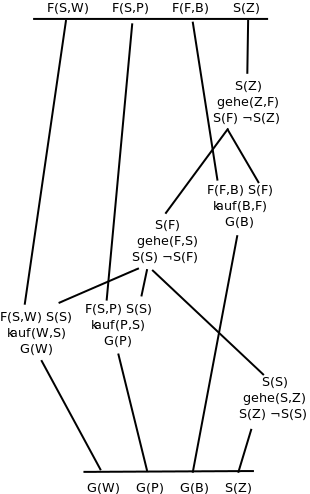
\includegraphics{planning.png} \\ \end{center}
    \item Der erstellte Plan erlaubt die Pralinen und den Wein im Supermarkt in beliebiger Reihnfolge zu kaufen.
\end{enumerate}
\end{document}
